
\documentclass[border=10pt, 12pt]{standalone}
\usepackage[svgnames]{xcolor}
\usepackage{amsmath}
\usepackage{pgfplots}
\pgfplotsset{compat=newest}
\usepackage[sfdefault]{FiraSans}
\usepackage{FiraMono}
\renewcommand*\familydefault{\sfdefault}
\begin{document}
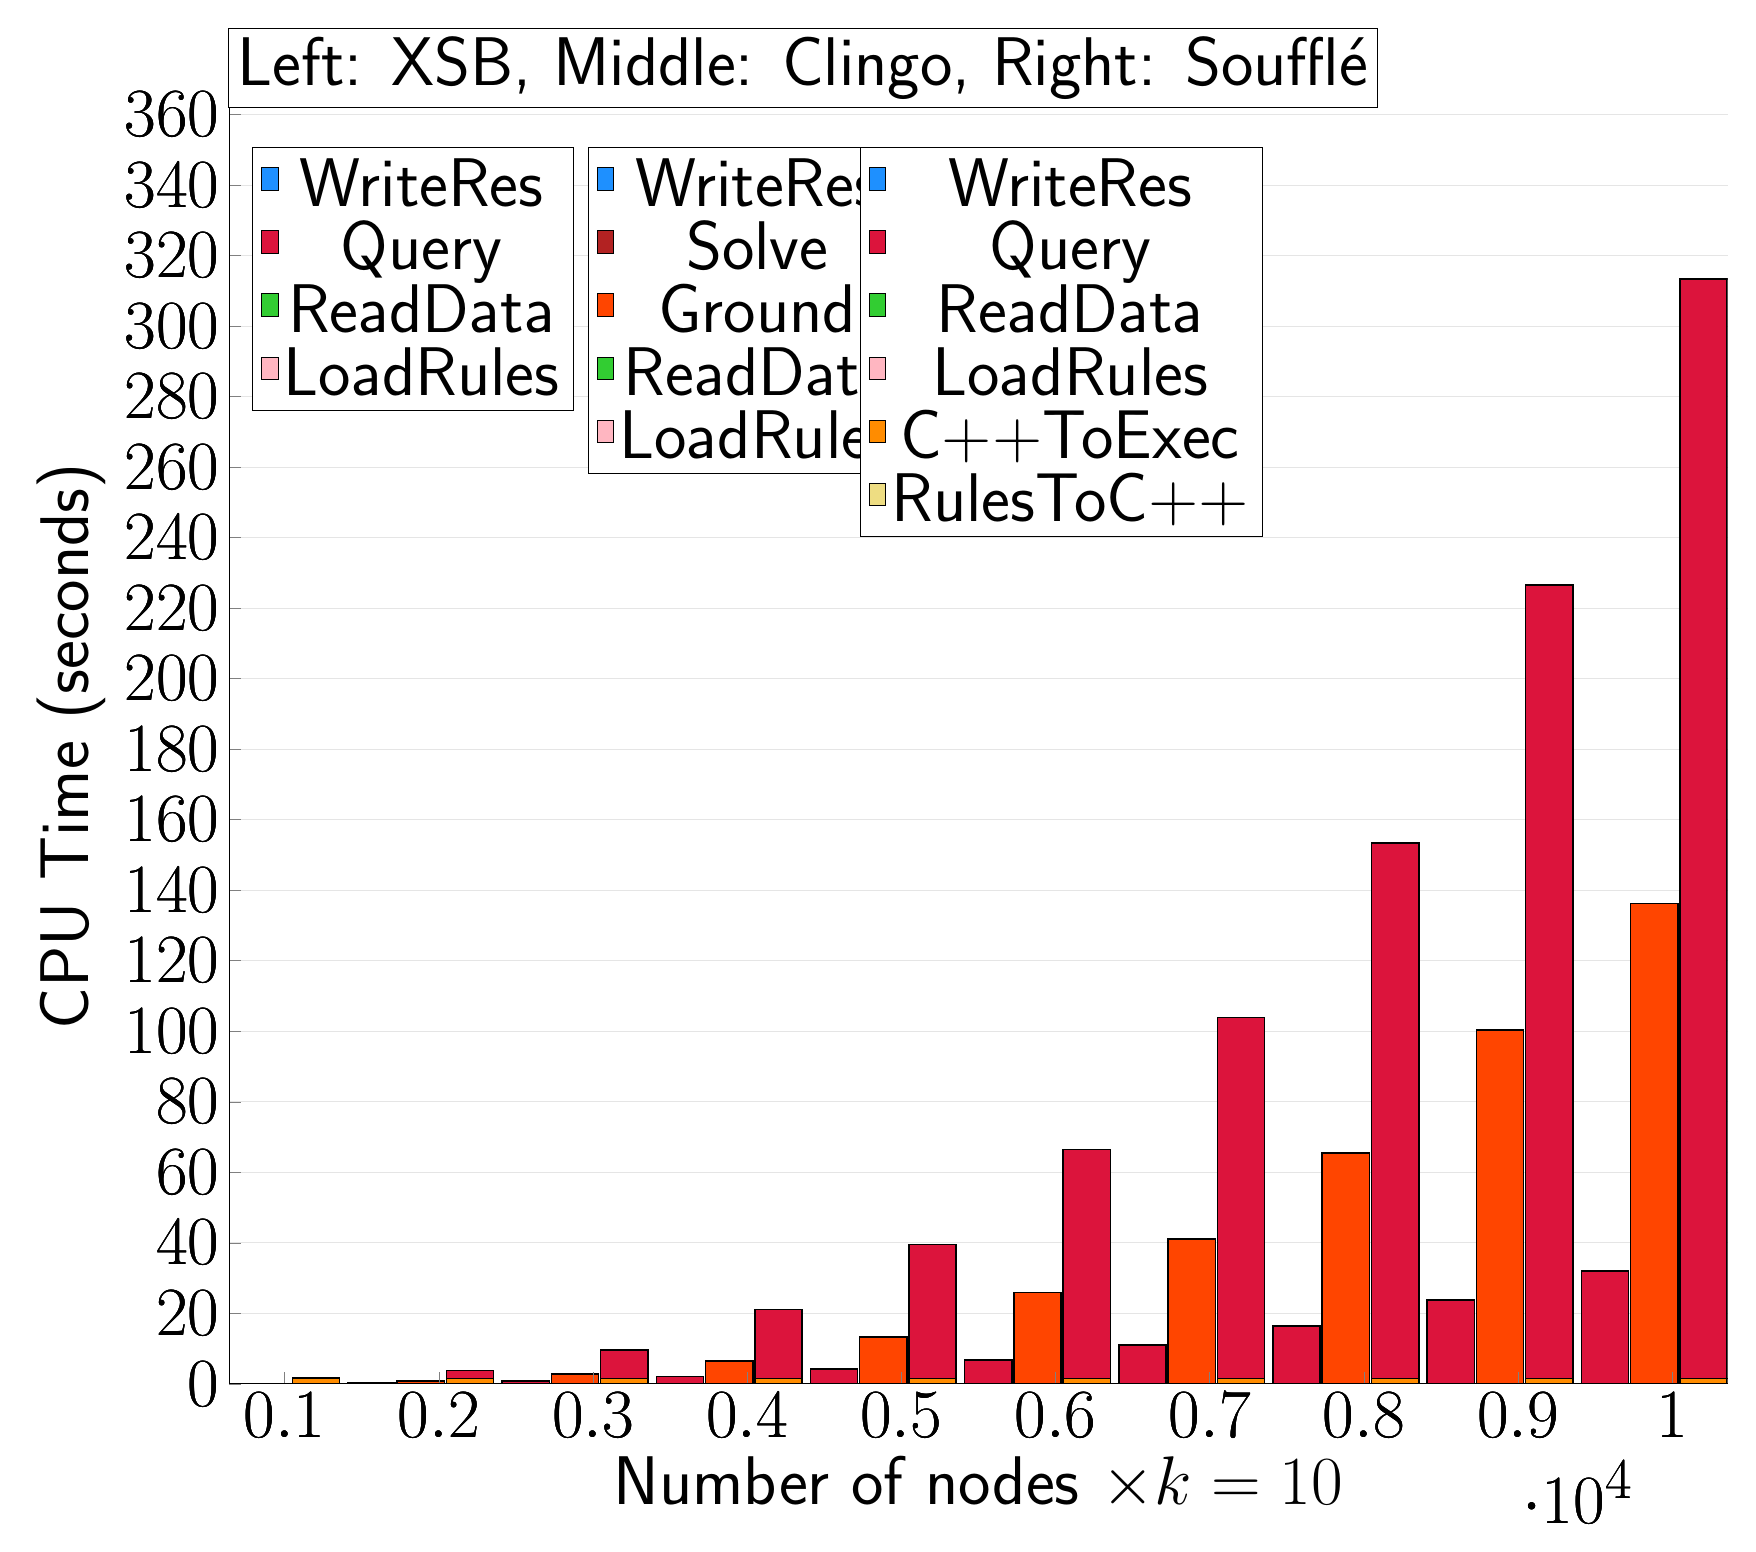
\begin{tikzpicture}
                        \begin{axis}[bar shift=-24.3pt, 
   ybar stacked,
   width=1.7\textwidth,
   bar width=0.6cm,
   ymajorgrids, tick align=inside,
   major grid style={draw=gray!20},
   xtick=data,
   ymin=0, ymax=361.7732,
   axis x line*=bottom,
   axis y line*=left,
   enlarge x limits=0.04,
   legend style={
       at={(0.23, 0.97)},
       anchor=north east,
       legend columns=1,
       font=\Huge,
   },
   ylabel={CPU Time (seconds)},
   xlabel={Number of nodes $\times k=10$},
   label style={font=\Huge},
   tick label style={font=\Huge},
]
\addlegendimage{fill=DodgerBlue, draw=black, line width=0.2pt}
\addlegendentry{WriteRes}
\addlegendimage{fill=Crimson, draw=black, line width=0.2pt}
\addlegendentry{Query}
\addlegendimage{fill=LimeGreen, draw=black, line width=0.2pt}
\addlegendentry{ReadData}
\addlegendimage{fill=LightPink, draw=black, line width=0.2pt}
\addlegendentry{LoadRules}
\addplot +[fill=LightPink, draw=black, line width=0.55pt] coordinates {
(1000, 0.0005537999999999999)
(2000, 0.0005591999999999995)
(3000, 0.0005555999999999998)
(4000, 0.0005532)
(5000, 0.0005524000000000002)
(6000, 0.0005510000000000001)
(7000, 0.0005539999999999992)
(8000, 0.0005522000000000003)
(9000, 0.0005635999999999995)
(10000, 0.0005619999999999996)
};
\addplot +[fill=LimeGreen, draw=black, line width=0.55pt] coordinates {
(1000, 0.0009629999999999994)
(2000, 0.0018352)
(3000, 0.0026958)
(4000, 0.0035778)
(5000, 0.0044562)
(6000, 0.0053014)
(7000, 0.006224)
(8000, 0.007076600000000001)
(9000, 0.007985599999999999)
(10000, 0.008846999999999999)
};
\addplot +[fill=Crimson, draw=black, line width=0.55pt] coordinates {
(1000, 0.0307178)
(2000, 0.2593906)
(3000, 0.8389634000000001)
(4000, 2.0705314)
(5000, 4.162048)
(6000, 6.744189399999999)
(7000, 11.0515688)
(8000, 16.3325292)
(9000, 23.7326566)
(10000, 31.857114000000003)
};
\addplot +[fill=DodgerBlue, draw=black, line width=0.55pt] coordinates {
(1000, 4.8400000000000526e-05)
(2000, 9.40000000000385e-06)
(3000, -0.00029360000000000497)
(4000, 0.0009087999999999319)
(5000, -0.005618000000000301)
(6000, -0.026816600000000256)
(7000, -0.07574699999999943)
(8000, -0.003540399999999977)
(9000, 0.0818169999999995)
(10000, 0.1756602000000008)
};
\end{axis}

\begin{axis}[bar shift=-6.5pt, 
   ybar stacked,
   width=1.7\textwidth,
   bar width=0.6cm,
   ymajorgrids, tick align=inside,
   major grid style={draw=none},
   xtick=data,
   ymin=0, ymax=361.7732,
   axis x line*=none,
   axis y line*=none,
   enlarge x limits=0.04,
   legend style={
       at={(0.454, 0.97)},
       anchor=north east,
       legend columns=1,
       font=\Huge,
   },
   label style={font=\Huge},
   tick label style={font=\Huge},
]
\addlegendimage{fill=DodgerBlue, draw=black, line width=0.2pt}
\addlegendentry{WriteRes}
\addlegendimage{fill=FireBrick, draw=black, line width=0.2pt}
\addlegendentry{Solve}
\addlegendimage{fill=OrangeRed, draw=black, line width=0.2pt}
\addlegendentry{Ground}
\addlegendimage{fill=LimeGreen, draw=black, line width=0.2pt}
\addlegendentry{ReadData}
\addlegendimage{fill=LightPink, draw=black, line width=0.2pt}
\addlegendentry{LoadRules}
\addplot +[fill=LightPink, draw=black, line width=0.55pt] coordinates {
(1000, 0.0)
(2000, 0.0)
(3000, 0.0)
(4000, 0.0)
(5000, 0.0)
(6000, 0.0)
(7000, 0.0)
(8000, 0.0)
(9000, 0.0)
(10000, 0.0)
};
\addplot +[fill=LimeGreen, draw=black, line width=0.55pt] coordinates {
(1000, 0.001999999999999996)
(2000, 0.0)
(3000, 0.0)
(4000, 0.008000000000000002)
(5000, 0.010000000000000009)
(6000, 0.01200000000000001)
(7000, 0.018000000000000016)
(8000, 0.020000000000000018)
(9000, 0.020000000000000018)
(10000, 0.020000000000000018)
};
\addplot +[fill=OrangeRed, draw=black, line width=0.55pt] coordinates {
(1000, 0.09800000000000003)
(2000, 0.782)
(3000, 2.7380000000000004)
(4000, 6.5200000000000005)
(5000, 13.213999999999999)
(6000, 25.832)
(7000, 41.122)
(8000, 65.41)
(9000, 100.39999999999999)
(10000, 136.2)
};
\addplot +[fill=FireBrick, draw=black, line width=0.55pt] coordinates {
(1000, 0.0)
(2000, 0.0020000000000000018)
(3000, 0.0)
(4000, 0.0)
(5000, 0.0019999999999999575)
(6000, 0.0)
(7000, 0.003999999999999204)
(8000, 0.006000000000000227)
(9000, 0.00600000000000307)
(10000, 0.004000000000002046)
};
\addplot +[fill=DodgerBlue, draw=black, line width=0.55pt] coordinates {
(1000, 0.0020000000000000018)
(2000, 0.001999999999999999)
(3000, 0.0)
(4000, 0.0)
(5000, -0.0019999999999999575)
(6000, 0.0020000000000003127)
(7000, -0.003999999999999204)
(8000, -0.006000000000000227)
(9000, -0.004000000000003068)
(10000, -0.0020000000000038654)
};
\end{axis}

\begin{axis}[bar shift=11.3pt, 
   ybar stacked,
   width=1.7\textwidth,
   bar width=0.6cm,
   ymajorgrids, tick align=inside,
   major grid style={draw=none},
   xtick=data,
   ymin=0, ymax=361.7732,
   axis x line*=none,
   axis y line*=none,
   enlarge x limits=0.04,
   legend style={
       at={(0.69, 0.97)},
       anchor=north east,
       legend columns=1,
       font=\Huge,
   },
   label style={font=\Huge},
   tick label style={font=\Huge},
]
\addlegendimage{fill=DodgerBlue, draw=black, line width=0.2pt}
\addlegendentry{WriteRes}
\addlegendimage{fill=Crimson, draw=black, line width=0.2pt}
\addlegendentry{Query}
\addlegendimage{fill=LimeGreen, draw=black, line width=0.2pt}
\addlegendentry{ReadData}
\addlegendimage{fill=LightPink, draw=black, line width=0.2pt}
\addlegendentry{LoadRules}
\addlegendimage{fill=DarkOrange, draw=black, line width=0.2pt}
\addlegendentry{C++ToExec}
\addlegendimage{fill=LightGoldenrod, draw=black, line width=0.2pt}
\addlegendentry{RulesToC++}
\addplot +[fill=LightGoldenrod, draw=black, line width=0.55pt] coordinates {
(1000, 0.004000000000000001)
(2000, 0.006000000000000001)
(3000, 0.008000000000000002)
(4000, 0.008000000000000002)
(5000, 0.006000000000000001)
(6000, 0.006000000000000001)
(7000, 0.0020000000000000005)
(8000, 0.0020000000000000005)
(9000, 0.0020000000000000005)
(10000, 0.001999999999999996)
};
\addplot +[fill=DarkOrange, draw=black, line width=0.55pt] coordinates {
(1000, 1.5099999999999998)
(2000, 1.514)
(3000, 1.52)
(4000, 1.52)
(5000, 1.5220000000000002)
(6000, 1.528)
(7000, 1.5219999999999998)
(8000, 1.522)
(9000, 1.516)
(10000, 1.5219999999999998)
};
\addplot +[fill=LightPink, draw=black, line width=0.55pt] coordinates {
(1000, 0.00015999999999999999)
(2000, 0.0001644)
(3000, 0.00015480000000000002)
(4000, 0.0001656)
(5000, 0.000157)
(6000, 0.00016900000000000002)
(7000, 0.00016860000000000003)
(8000, 0.00019979999999999998)
(9000, 0.0001774)
(10000, 0.00017300000000000003)
};
\addplot +[fill=LimeGreen, draw=black, line width=0.55pt] coordinates {
(1000, 0.0042884)
(2000, 0.0076359999999999996)
(3000, 0.0101576)
(4000, 0.013605800000000001)
(5000, 0.0157264)
(6000, 0.0194332)
(7000, 0.0217358)
(8000, 0.0250378)
(9000, 0.026451199999999998)
(10000, 0.0282132)
};
\addplot +[fill=Crimson, draw=black, line width=0.55pt] coordinates {
(1000, 0.3129178)
(2000, 2.197934)
(3000, 8.094296)
(4000, 19.592080000000003)
(5000, 38.0132)
(6000, 64.8875)
(7000, 102.3916)
(8000, 151.9096)
(9000, 224.99960000000002)
(10000, 311.7732)
};
\addplot +[fill=DodgerBlue, draw=black, line width=0.55pt] coordinates {
(1000, 0.0002926)
(2000, 0.0004556)
(3000, 0.0004208)
(4000, 0.0004568)
(5000, 0.00044219999999999996)
(6000, 0.00035839999999999993)
(7000, 0.0004142)
(8000, 0.0004638)
(9000, 0.0005671999999999999)
(10000, 0.000515)
};
\end{axis}


\node[anchor=south, draw, fill=white] at (rel axis cs:0.42,1) {\Huge Left: XSB, Middle: Clingo, Right: Soufflé};
\end{tikzpicture}
\end{document}
                    